\documentclass[11pt]{article}
\usepackage[a4paper, left=1in, right=1in, top=1in, bottom=1in]{geometry}
\usepackage{graphicx}
\usepackage[small]{titlesec}
\usepackage{amsmath,amssymb}
\usepackage[utf8]{inputenc}
\usepackage[T1]{fontenc}
\usepackage[english]{babel}
\usepackage[tikz]{mdframed}
\usepackage{float}
\usepackage{multirow}
\usepackage{hyperref}
\usepackage{xcolor}
\usepackage[numbers]{natbib}
\hypersetup{
    colorlinks=true,
    linkcolor=orange,
    urlcolor=orange,
    citecolor=orange
}

\title{Leveraging Short-Term, Map-Specific Player Statistics for Counter-Strike 2 Match Prediction }

\author{}

\date{April 14, 2025 \\ \small Revised October 8, 2026}

% \setcounter{section}{-1}
\begin{document}

\maketitle

\begin{abstract}
This project explores the prediction of Counter-Strike 2 (CS2) match outcomes using machine learning techniques, with a focus on short-term (90-day), map-specific player performance metrics. Player statistics are aggregated into team-level features, and the performance of TabPFN - a Transformer-based meta-learning model - is evaluated against tuned classical models including logistic regression, XGBoost, and LightGBM. Across 30 repeated held-out splits the models reach about 72\% accuracy and an AUC of 0.80, and the result holds when training on older matches and testing on newer ones. A two-feature logistic regression on team rating and map win-rate differences captures most of this signal, and an apparent gain from feature pruning disappears once the features are selected without using the test set.
\end{abstract}

\begin{mdframed}
\small\textbf{Revision note (October 2026).} The original version of this report (April 2025) contained several errors, corrected here: (1) the headline results for pruned LightGBM (79.7\% accuracy) and pruned XGBoost (77.7\%) used features selected with permutation importance computed on the test set, which makes them optimistic; (2) the 95\% confidence interval in Section~4.1 was computed with the full dataset size instead of the 202-map test set; (3) the dataset contains 1010 maps from 577 matches, not 1010 unique matches; (4) one citation named the wrong authors. Section~7 is new: it re-evaluates the models over repeated and forward-in-time splits and against a simple two-feature baseline. The original single-split tables and figures are kept unchanged. All new numbers are reproducible with \texttt{robustness\_check.py} in the project repository.
\end{mdframed}

\tableofcontents
\newpage
\section{Introduction}
The primary objective of this project is to develop a predictive model for Counter-Strike 2 match outcomes that outperforms existing public models. The central research question is: Can a novel data representation strategy, combined with the state-of-the-art TabPFN model, yield significantly higher predictive accuracy on HLTV-derived Counter-Strike 2 data than existing models?

Our approach centres on restructuring input data to emphasize recent player performance on a per-map basis, rather than relying on long-term aggregate statistics. This refinement is motivated by the hypothesis that short-term, map-specific performance trends are more predictive of upcoming match outcomes, particularly in the context of Counter-Strike 2, where team dynamics and player form can vary substantially across space and time.

Although prior work has explored Counter-Strike: Global-Offensive and Counter-Strike 2 match prediction using conventional machine learning models, to the best of our knowledge, no study has yet evaluated the performance of TabPFN - a recently released Transformer-based probabilistic meta-learning model - on esports data. This project introduces novelty in both model selection and evaluation: we benchmark TabPFN against a tuned ensemble of classical models, including logistic regression, XGBoost, and LightGBM. This modelling strategy, combined with our domain-specific feature engineering - centered on short-term, map-aware player metrics - represents a methodological contribution to the field of Counter-Strike 2 esports analytics.

The primary aim of this work is to test how far publicly available data can go in predicting Counter-Strike 2 match outcomes. The project applies recent advances in meta-learning to a new domain and examines whether performance-aware feature construction improves match forecasting. Accurate prediction of CS2 match outcomes is relevant to analysts, teams, and fans who rely on performance forecasting.

\section{Background}
Counter-Strike 2 (CS2) is a competitive round-based first-person shooter that serves as the successor to Counter-Strike: Global Offensive (CS:GO). In professional esports settings, CS2 matches are played in structured formats such as best-of-one (Bo1), best-of-three (Bo3), or best-of-five (Bo5) series, where teams compete to be the first to win 13 rounds and thus earning them an individual map win. A central feature of competitive CS2 is its map pool - a curated set of playable maps each having a unique geometric layout allowing for different play-styles of players to shine through. Thus, team’s or player’s effectiveness is not solely a function of their overall skill, but also of their compatibility with the specific tactical demands of a given map. This gives rise to the concept of map-specific performance which takes into account not the aggregated statistics of a player across all recent maps but rather a specific one. Typical metrics used to characterize player performance include: kills, deaths, kill/death ratio, headshot percentage, damage per round, and their overall rating (Rating 2.0) which is calculated by HLTV using above metrics and many more.

The required data needed for this project is largely accessible through HLTV, a news website and forum which covers professional CS2 esports news, tournaments, and statistics such as individual player performance metrics and team performance metrics.
\section{Literature Review}
Previous studies have explored the use of machine learning to predict outcomes of professional Counter-Strike matches, focusing primarily on CS:GO - the predecessor to the more recently released CS2 - by leveraging statistical data from platforms such as HLTV. One of the most comprehensive studies is by Tabacof~\cite{tabacof2023csgo}, who developed a model using LightGBM trained on over 30,000 professional matches with extensive feature engineering, including Bayesian TrueSkill ratings. His approach achieved high predictive performance with a reported accuracy of 70.1\% and AUC of 0.773 on an out-of-time test set, making it one of the most effective pre-match models to date. The study included a brief feature importance analysis although no actual feature selection in the form of permutation importance or adversarial validation was performed.

Similarly, Švec~\cite{svec2022csgo} conducted an extensive comparison of models using a dataset of over 40,000 matches. He evaluated several sample representations and models, including linear models, tree ensembles, and deep learning architectures. His best-performing model was based on a player-level Elo rating system, which achieved a test accuracy of 64\%, closely followed by a Random Forest model at 63\%. Švec's work also emphasized the importance of using round-based team and player statistics, and he experimented with CNNs and embedding-based neural networks, although their performance did not surpass simpler models.

Broms \& Nordansjö~\cite{broms2024cs} focused on logistic regression and tree-based models using a curated dataset of 3,788 matches from 2016-2020. Their LASSO-regularized logistic regression model achieved an accuracy of 60.5\%, with a Cohen's kappa of 0.21.
Other studies such as those by Makarov et al.~\cite{makarov2018predicting} and Xenopoulos et al.~\cite{xenopoulos2020valuing} have also contributed valuable insights, with models incorporating probabilistic skill ratings and in-game event streams achieving accuracy of 62\% and AUCs as high as 0.791. Overall, the literature consistently finds that performance metrics such as Elo, TrueSkill, and well-curated historical features are among the strongest predictors of match outcomes, with most models achieving predictive accuracies between 60\% and 65\%.

\section{Data and Feature Engineering}
The dataset used for this project was obtained via Kaggle~\cite{picinin2024hltv}, covering professional Counter-Strike 2 matches played between November 2023 and January 2024. In addition to match identifiers (matchID), team names, and the specific map played, the raw dataset included detailed player-level performance metrics for all ten participants, alongside team-level map win-rates. Crucially, all provided player and team statistics reflect performance specifically on the map being played, aggregated over the preceding 90 days.

Initial data cleaning involved removing rows with missing map information and excluding columns corresponding to the obsolete Rating 1.0 system (a legacy feature from CS:GO, superseded by Rating 2.0 in CS2). This preprocessing resulted in a dataset containing 1010 maps from 577 matches (a best-of-three match contributes one row for each map played), described by 147 initial features and a binary target column indicating the match winner. Of the 147 features, 140 represented player-specific statistics (14 distinct metrics per player), and two represented the map-specific win rates for each team. The 14 player-level metrics captured various aspects of performance, including: total kills, headshot percentage, total deaths, kill/death ratio, damage per round, grenade damage per round, maps played, rounds played, kills per round, assists per round, deaths per round, saves by teammate per round, saved teammates per round, and the overall HLTV Rating (Rating 2.0).
To create team-level representations capturing both aggregate performance and intra-team consistency, the 14 types of individual player statistics were aggregated within each five-player team. Specifically, for each metric type (e.g., kills, kill/death ratio), five summary statistics were computed across the team's players: the mean, standard deviation, sum, minimum, and maximum values. This aggregation process generated 70 derived statistical features per team (14 metrics with 5 aggregations per each), resulting in 140 team-based features across both competing teams per match. These 140 derived features were then combined with the two original team-specific map win-rate features.

Consequently, the final dataset prepared for modelling consisted of 1010 rows, each described by 142 predictive features. The target variable was encoded as a binary column, where a value of 1 indicated a win for the designated "Team 1", and 0 indicated a loss. Team 1 won 54.0\% of maps, so always predicting a Team 1 win gives a baseline accuracy of 54\%. This finalized dataset was subsequently partitioned into an 80\% training set and a 20\% test set to facilitate model training and evaluation.

\subsection{Preliminary Results}
To obtain an initial assessment of the predictive potential of the engineered features, a simple, untuned logistic regression model was trained. Evaluating this model on the test set it achieved an accuracy of 70.3\% and an AUC score of 0.782. This is similar to the 71\% accuracy reported by the author of the Kaggle dataset~\cite{picinin2024hltv}, and above the 60-65\% typical of prior CS:GO/CS2 studies. That comparison is not like-for-like: the prior studies used tens of thousands of matches and, in Tabacof's case, an out-of-time test set, whereas this dataset is small (1010 maps) and covers a narrow period (November 2023 - January 2024). A 95\% confidence interval for the accuracy, based on the 202 test maps, is [0.640, 0.766], so differences of a few percentage points between models on this test set are within sampling noise. Despite these considerations and the need for further validation, the encouraging preliminary performance motivated the decision to proceed with training more increasingly complex models, such as XGBoost, LightGBM, and TabPFN, utilizing the developed feature set.

\section{Research Plan and Methodology}
This study employs a comparative machine learning approach to evaluate predictive models for CS2 match outcomes, utilizing the feature set developed previously. The core methodology involves training and comparing several models, including both a baseline logistic regression and a version optimized via cross-validated hyperparameter tuning, exploring techniques such as regularization. Similarly, gradient boosting machines, specifically XGBoost and LightGBM, were evaluated by comparing baseline configurations against versions tuned using cross-validation. Furthermore, the state-of-the-art Transformer-based meta-learning model, TabPFN, was applied to assess its performance on this specific tabular esports dataset. The research process began with the data preparation steps of cleaning the dataset and implementing the feature engineering strategy detailed in Section 4. The selected models were then trained on the training partition of the data, using cross-validation on this partition to determine hyperparameters for the tunable models (Logistic Regression, XGBoost, LightGBM). All trained models were evaluated on the held-out test set using standard classification metrics, namely Accuracy, AUC, Log-Loss, and Average Precision. Feature importance was then analysed using L1 regularization coefficients and permutation importance, and these results were used for feature selection and retraining. The final stage was a comparative analysis of the developed models against each other.

\section{Results and Analysis}
\subsection{Logistic Regression}
A baseline logistic regression model was compared against a version optimized using cross-validated hyperparameter tuning. The tuning process identified L1 regularization (Lasso) as the most effective strategy. Lasso regularization performs inherent feature selection by shrinking the coefficients of less informative features towards zero. Consequently, examining the non-zero coefficients in the tuned model provides insight into feature relevance. Key predictors identified through this process included player Rating 2.0, deaths per round, and team-specific map win rates (Figure~\ref{fig:LassoCoef}).

As shown in Table~\ref{tab:logistic_regression_comparison_table}, the tuned model exhibited superior performance on the test set across all evaluation metrics compared to the baseline. Notably, accuracy increased by 3 percentage points, and improvements were also observed in the Area Under the ROC Curve (AUC) and Average Precision (AP), visualized in Figure~\ref{fig:logistic_regression_curve_comparisons}. Log-loss saw a marginal improvement, decreasing slightly.

Furthermore, analysis of the confusion matrices (Figure~\ref{fig:logistic_regression_confusion_matrices}) showed that the tuned model reduced the number of false positives (incorrectly predicting a win for "Team 1") from 32 to 27.

\begin{table}[H]
\centering
\begin{tabular}{lcccc}
\hline
\textbf{Model} & \textbf{Accuracy} & \textbf{AUC} & \textbf{Log-Loss} & \textbf{AP} \\
\hline
Basic Logistic Regressor       & 0.703 & 0.782 & 0.559 & 0.826 \\
Tuned Logistic Regressor       & 0.733 & 0.801 & 0.548 & 0.847 \\
\hline
\end{tabular}
\caption{Performance comparison of a basic and tuned logistic regression model on the test set, evaluated using Accuracy, AUC, Log-Loss, and AP.}
\label{tab:logistic_regression_comparison_table}
\end{table}

\begin{figure}[H]
    \centering
    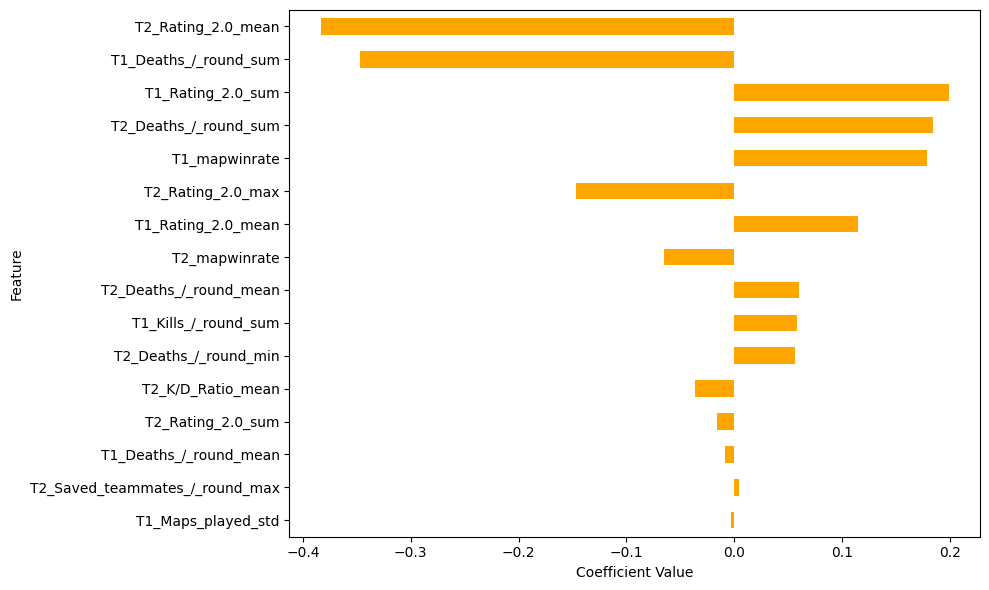
\includegraphics[width=0.8\linewidth]{LassoCoefficients.png}
    \caption{Non-zero feature coefficients from the tuned L1-regularized (Lasso) logistic regression model. Features with positive coefficients increase the predicted probability of Team 1 winning, while negative coefficients decrease it.}
    \label{fig:LassoCoef}
\end{figure}


\begin{figure}[H]
    \centering
    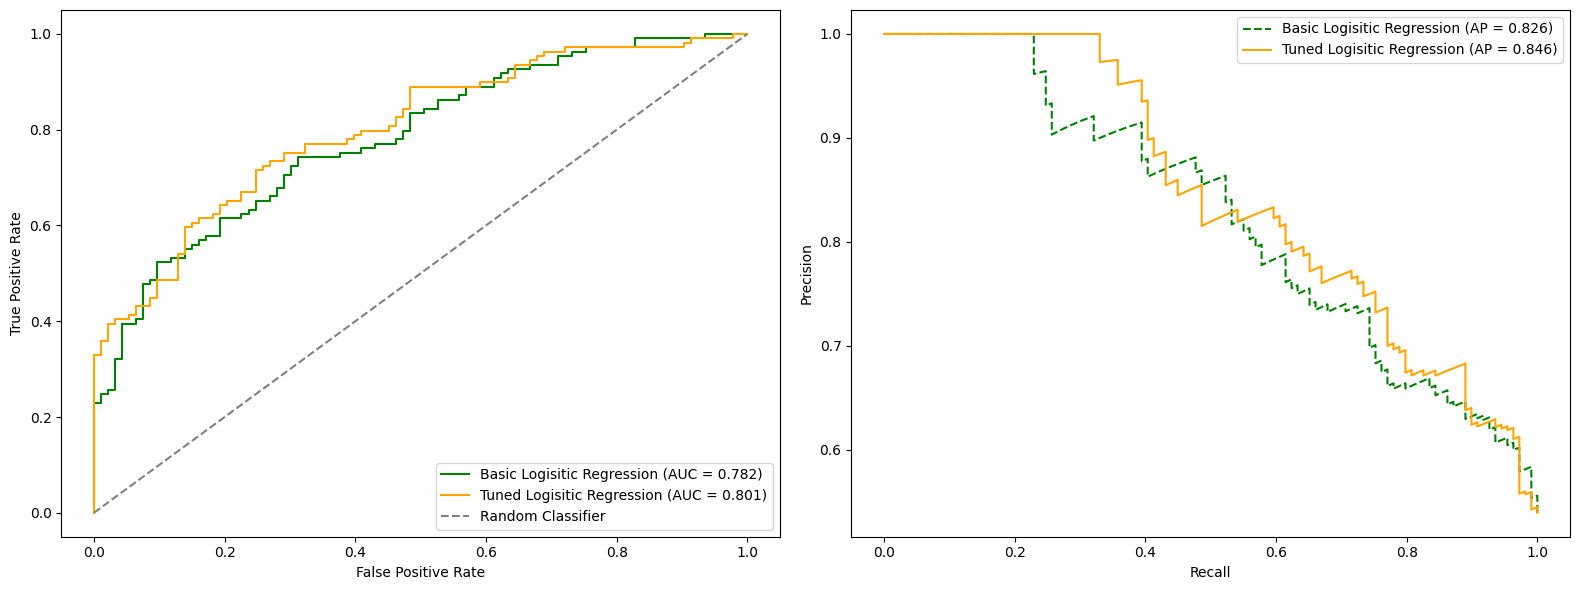
\includegraphics[width=1\linewidth]{logistic_regression_curve_comparisons.png}
    \caption{Performance curves comparing basic and tuned (Lasso) logistic regression models on the test set. Left: Receiver Operating Characteristic (ROC) curves showing True Positive Rate vs. False Positive Rate. Right: Precision-Recall (PR) curves. Area Under Curve (AUC) and Average Precision (AP) scores are indicated in the legends.}
    \label{fig:logistic_regression_curve_comparisons}
\end{figure}


\begin{figure}[H]
    \centering
    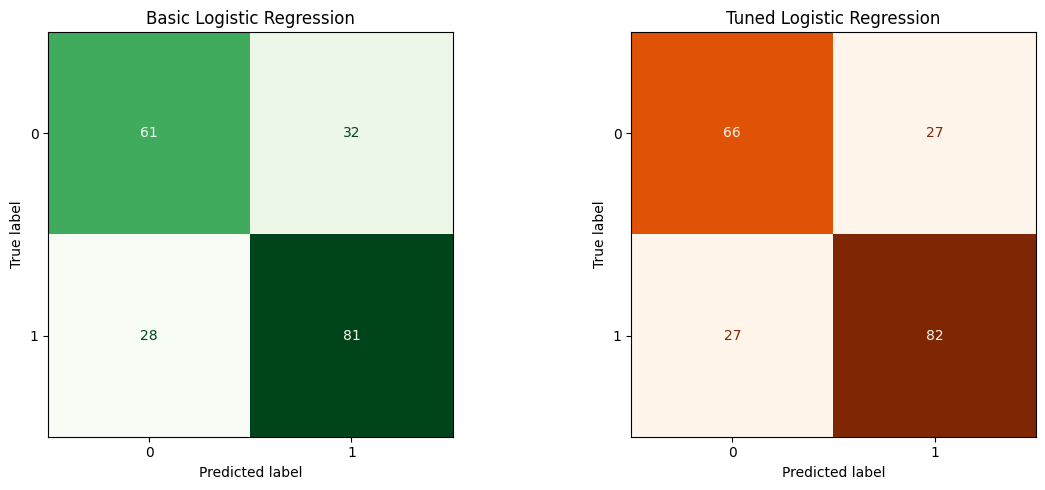
\includegraphics[width=1\linewidth]{logistic_regression_confusion_matrices.png}
    \caption{Comparison of confusion matrices for the basic (left) and tuned (Lasso, right) logistic regression models on the test set. Values indicate counts for True Negatives (top-left), False Positives (top-right), False Negatives (bottom-left), and True Positives (bottom-right).}
    \label{fig:logistic_regression_confusion_matrices}
\end{figure}

\subsection{LightGBM}
The performance of three LightGBM model variations was evaluated: a baseline configuration, a version tuned using cross-validated hyperparameter optimization, and a final version trained on a pruned feature set identified via permutation importance.

Compared to the baseline model, hyperparameter tuning yielded slight improvements in Accuracy, AUC, and AP on the test set, although it resulted in a higher Log-Loss (Table~\ref{tab:LightGBM_comparison_table} and Figure \ref{fig:lightgbm_curves_comparison}). To reduce model complexity, permutation feature importance was calculated using the tuned model on the test set. Features contributing below a predefined importance threshold were subsequently removed.

A new LightGBM model was then trained using only this reduced feature set. Because the features were chosen using the same test set the model is scored on, the pruned results in Table~\ref{tab:LightGBM_comparison_table} are optimistic; Section~7 repeats the pruning with features chosen on training data only, where the gain disappears. On the original test set, this 'pruned' model demonstrated markedly superior performance compared to both the basic and tuned versions across all metrics, achieving the highest Accuracy, AUC, and AP, along with the lowest Log-Loss (Table~\ref{tab:LightGBM_comparison_table}). The confusion matrices further illustrate this enhanced predictive capability, showing a clear increase in correctly classified instances and a reduction in false positives for the pruned model (Figure~\ref{fig:lightgbm_confusion_matrices.png}).

Analysis of the feature importances derived from the permutation process (Figure~\ref{fig:feature_importance_lightgbm}) indicated that the kill/death ratio was a highly influential predictor, despite exhibiting considerable variability across permutations reflected in its standard deviation. Other features demonstrating significant predictive value included the teams' map-specific win rates and deaths per round.

\begin{table}[H]
\centering
\begin{tabular}{lcccc}
\hline
\textbf{Model} & \textbf{Accuracy} & \textbf{AUC} & \textbf{Log-Loss} & \textbf{AP} \\
\hline
Basic LightGBM       & 0.728 & 0.814 & 0.657 & 0.844 \\
Tuned LightGBM       & 0.733 & 0.815 & 0.746 & 0.852 \\
Pruned LightGBM$^\dagger$ & 0.797 & 0.862 & 0.569 & 0.889 \\
\hline
\end{tabular}
\caption{Performance comparison of a basic, tuned, and pruned LightGBM model on the test set, evaluated using Accuracy, AUC, Log-Loss, and AP. $^\dagger$Features selected using the test set; optimistic (see Section~7).}
\label{tab:LightGBM_comparison_table}
\end{table}

\begin{figure}[H]
    \centering
    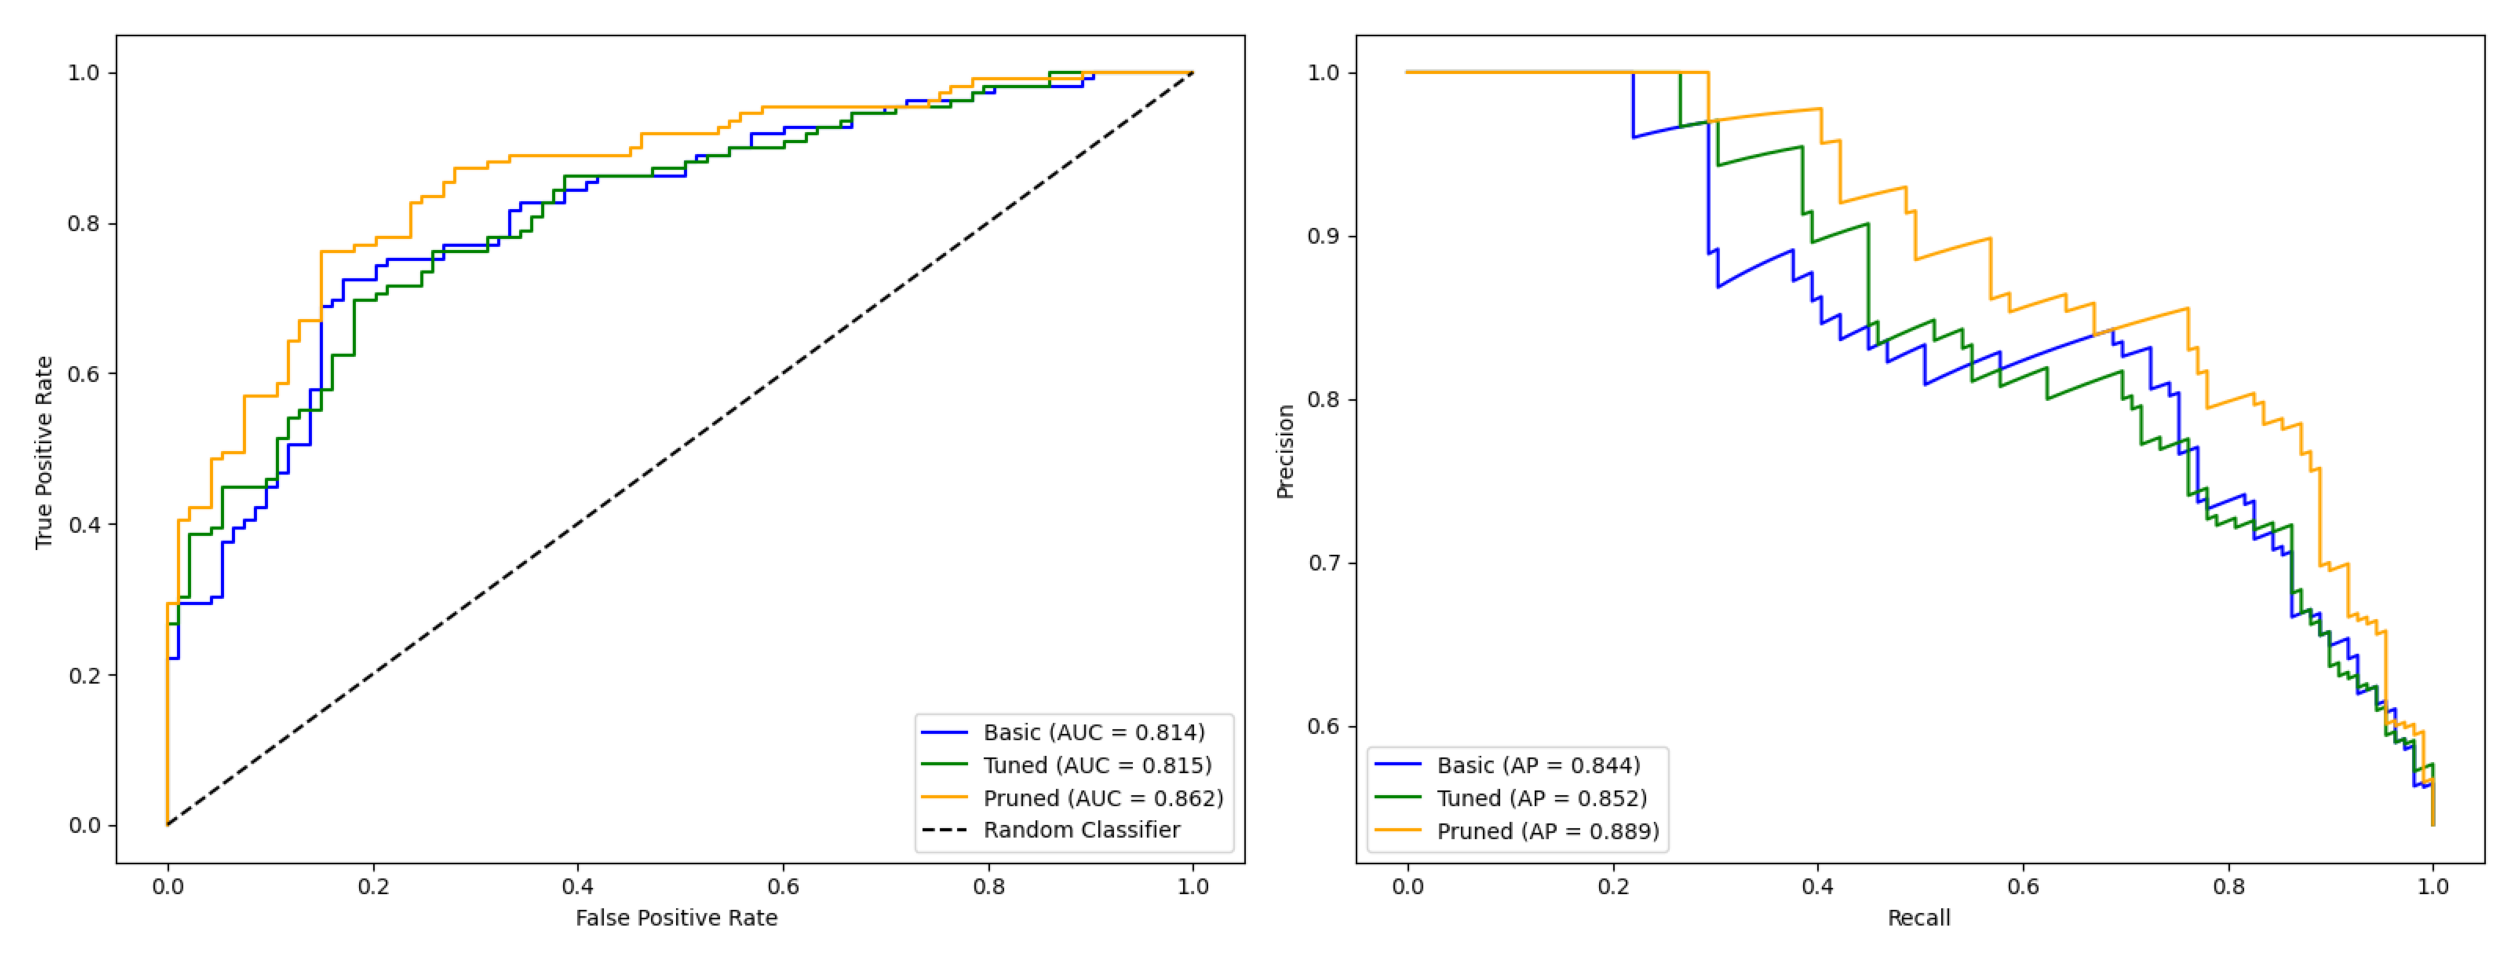
\includegraphics[width=1\linewidth]{lightgbm_curves_comparison.png}
    \caption{Performance curves comparing basic, tuned, and pruned LightGBM models on the test set. Left: ROC curves. Right: PR curves. AUC and AP scores are indicated in the legends for each model variation.}
    \label{fig:lightgbm_curves_comparison}
\end{figure}

\begin{figure}[H]
    \centering
    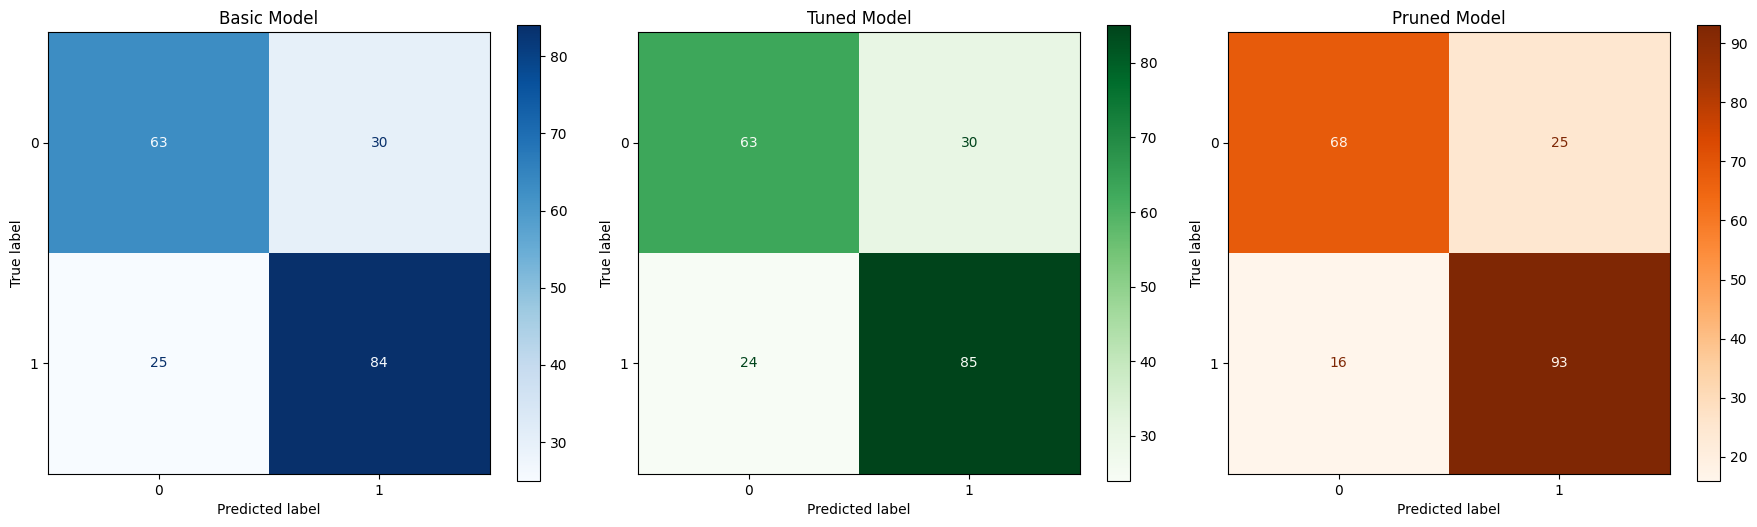
\includegraphics[width=1\linewidth]{lightgbm_confusion_matrices.png}
    \caption{Comparison of confusion matrices for the basic (left), tuned (center), and pruned (right) LightGBM models on the test set. Values indicate counts for True Negatives (top-left), False Positives (top-right), False Negatives (bottom-left), and True Positives (bottom-right).}
    \label{fig:lightgbm_confusion_matrices.png}
\end{figure}

\begin{figure}[H]
    \centering
    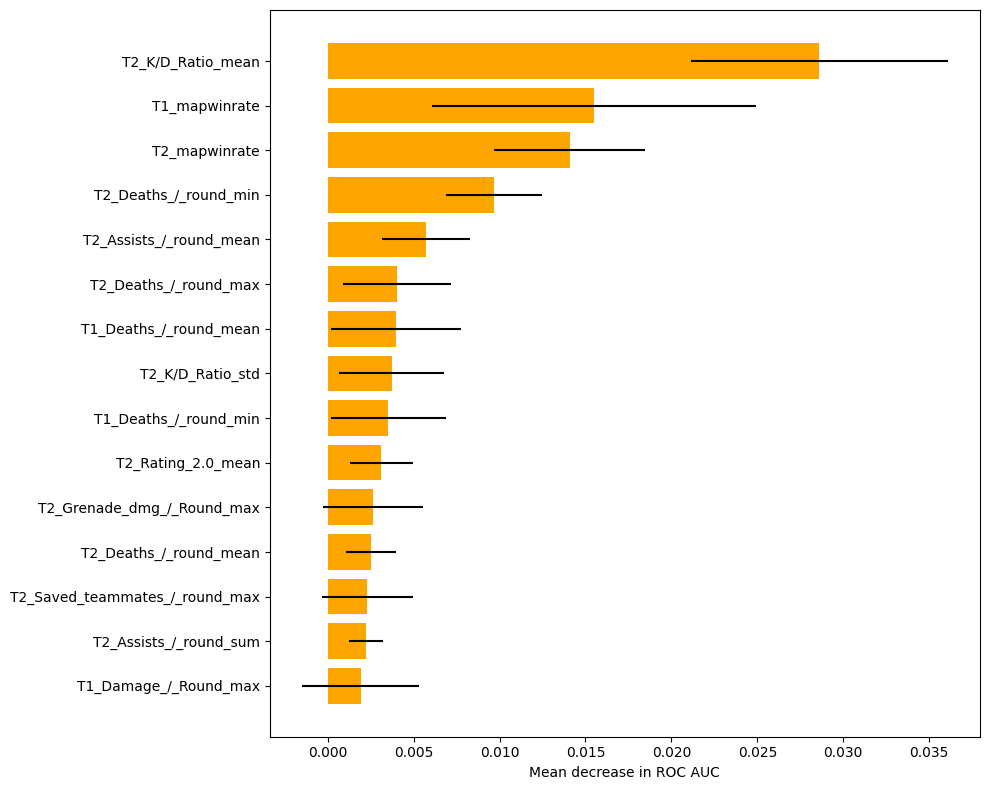
\includegraphics[width=0.7\linewidth]{feature_importance_lightgbm.png}
    \caption{Top 15 features ranked by permutation importance for the tuned LightGBM model. Importance is measured as the mean decrease in test set ROC AUC when the feature's values are randomly permuted. Error bars indicate the standard deviation across permutations.}
    \label{fig:feature_importance_lightgbm}
\end{figure}


\subsection{XGBoost}
Evaluation of the XGBoost models followed a similar three-stage process: comparing a baseline configuration, a version optimized via cross-validated hyperparameter tuning, and a final model trained on a pruned feature set.

As detailed in Table~\ref{tab:XGBoost_comparison_table}, hyperparameter tuning improved the model's performance over the baseline on AUC, Log-Loss, and AP when evaluated on the test set (Figure \ref{fig:XGBoost_curves_comparison}). However, this came at the cost of a slight decrease in accuracy.

To explore potential improvements through feature selection, permutation importance was computed using the tuned model on the test set. Features falling below a set importance threshold were subsequently removed. An XGBoost model retrained using only this reduced feature set achieved the highest performance across all evaluated metrics on the test set, with an accuracy of 77.7\% and an AUC of 0.834. As with LightGBM, these pruned scores are optimistic because the test set was used to choose the features.

The feature importance analysis itself highlighted team-specific map win-rates, deaths per round, and kill/death ratio as being among the most influential predictors for the XGBoost model (Figure~\ref{fig:XGBoost_permutation_importance}). Correspondingly, the confusion matrix for the pruned model demonstrated a pronounced increase in correct classifications compared to the non-pruned versions, accompanied by a modest reduction in the number of false positives (Figure~\ref{fig:XGBoost_confusion_matrices}).

\begin{table}[H]
\centering
\begin{tabular}{lcccc}
\hline
\textbf{Model} & \textbf{Accuracy} & \textbf{AUC} & \textbf{Log-Loss} & \textbf{AP} \\
\hline
Basic XGBoost       & 0.733 & 0.799 & 0.558 & 0.830 \\
Tuned XGBoost       & 0.719 & 0.815 & 0.536 & 0.850 \\
Pruned XGBoost$^\dagger$ & 0.777 & 0.834 & 0.513 & 0.871 \\
\hline
\end{tabular}
\caption{Performance comparison of a basic, tuned, and pruned XGBoost model on the test set, evaluated using Accuracy, AUC, Log-Loss, and AP. $^\dagger$Features selected using the test set; optimistic (see Section~7).}
\label{tab:XGBoost_comparison_table}
\end{table}

\begin{figure}[H]
    \centering
    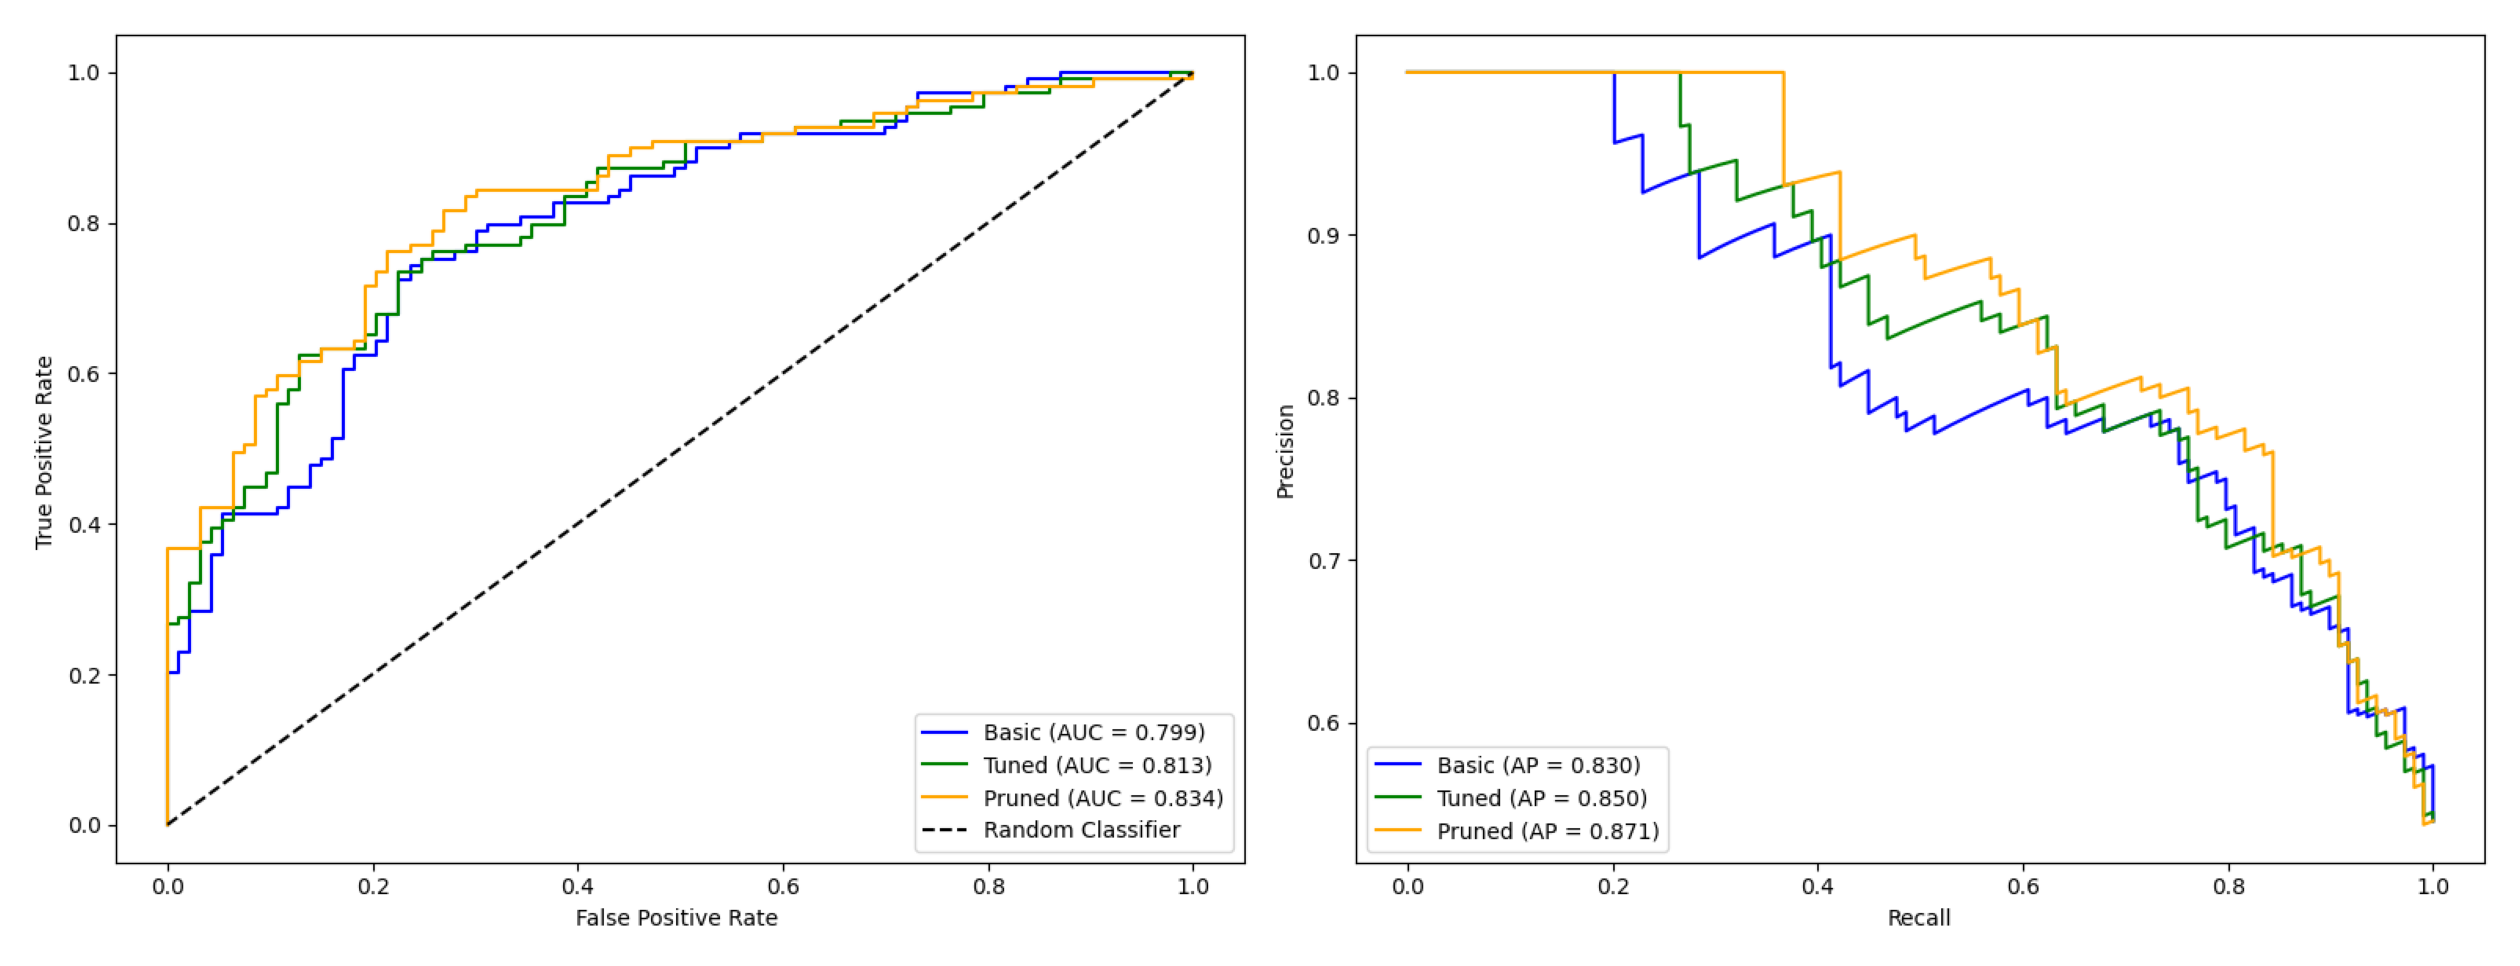
\includegraphics[width=1\linewidth]{XGBoost_curves_comparison.png}
    \caption{Performance curves comparing basic, tuned, and pruned XGBoost models on the test set. Left: ROC curves. Right: PR curves. AUC and AP scores are indicated in the legends for each model variation.}
    \label{fig:XGBoost_curves_comparison}
\end{figure}

\begin{figure}[H]
    \centering
    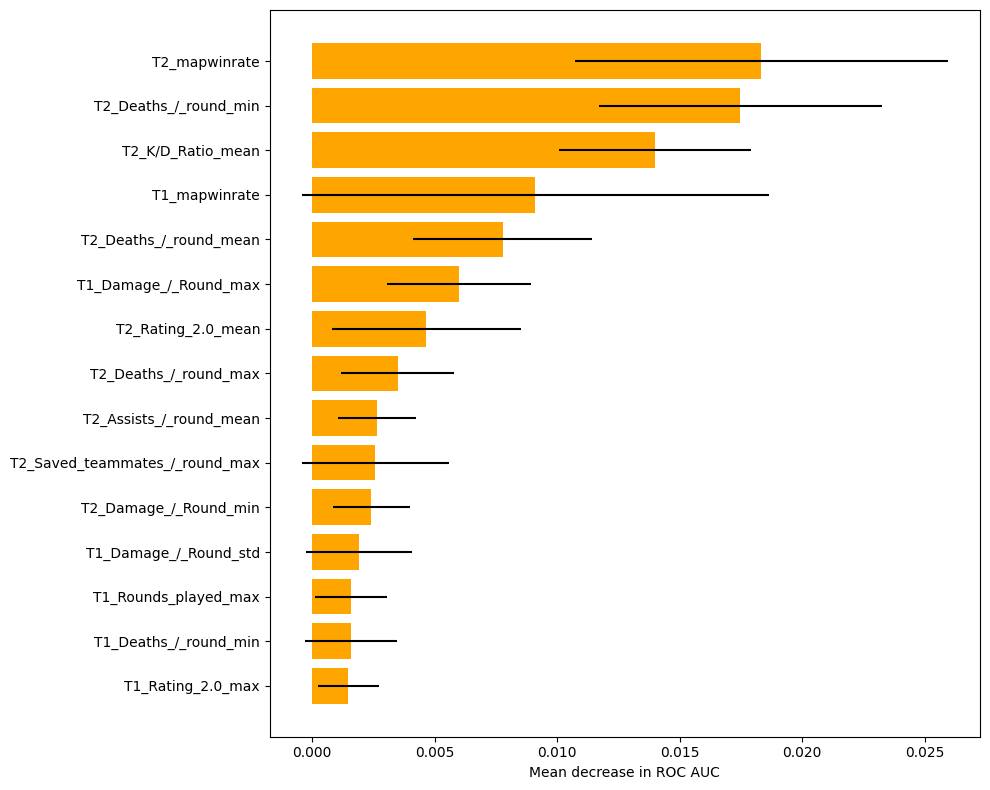
\includegraphics[width=0.7\linewidth]{XGBoost_permutation_importance.png}
    \caption{Top 15 features ranked by permutation importance for the tuned XGBoost model. Importance is measured as the mean decrease in test set ROC AUC when the feature's values are randomly permuted. Error bars show the standard deviation across permutations.}
    \label{fig:XGBoost_permutation_importance}
\end{figure}

\begin{figure}[H]
    \centering
    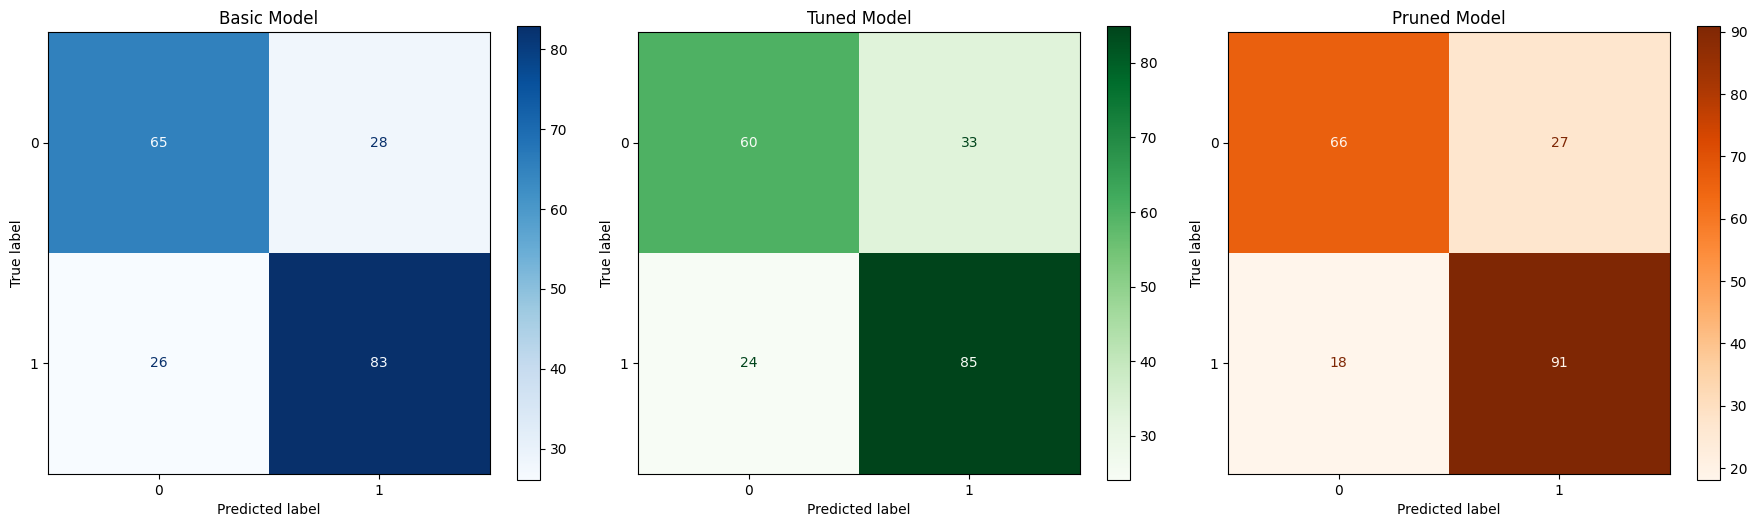
\includegraphics[width=1\linewidth]{XGBoost_confusion_matrices.png}
    \caption{Comparison of confusion matrices for the basic (left), tuned (centre), and pruned (right) XGBoost models on the test set. Values indicate counts for True Negatives (top-left), False Positives (top-right), False Negatives (bottom-left), and True Positives (bottom-right).}
    \label{fig:XGBoost_confusion_matrices}
\end{figure}

\subsection{TabPFN}
TabPFN operates differently from the tree-based models evaluated, as a pre-trained transformer designed for tabular data, it achieves strong performance without requiring hyperparameter tuning \cite{hollmann2025accurate}. We evaluated TabPFN under four distinct scenarios: firstly, using the complete set of 142 engineered features, and subsequently, using three pruned feature subsets derived from the feature importance analyses previously conducted for the tuned Logistic Regression, LightGBM, and XGBoost models. The LightGBM and XGBoost subsets were chosen using test-set permutation importance, so those two rows share the optimism described above.

The performance of these TabPFN configurations on the test set is detailed in Table~\ref{tab:TabPFN_comparison_table}. Employing the feature subsets derived from Logistic Regression or XGBoost resulted in a noticeable degradation across all evaluation metrics compared to the baseline TabPFN model using the full feature set.

Conversely, applying TabPFN with the feature subset identified as most important by LightGBM yielded a marginal increase in accuracy (from 73.3\% to 74.3\%). However, this improvement was accompanied by an identical AUC score (0.835) and slight decreases in performance for Log-Loss (0.487 to 0.489) and AP (0.875 to 0.867). Analysis of the confusion matrices indicated that using this LightGBM-derived feature subset resulted in a minuscule improvement (Figure \ref{fig:TabPFN_confusion_matrices}).


\begin{figure}[H]
    \centering
    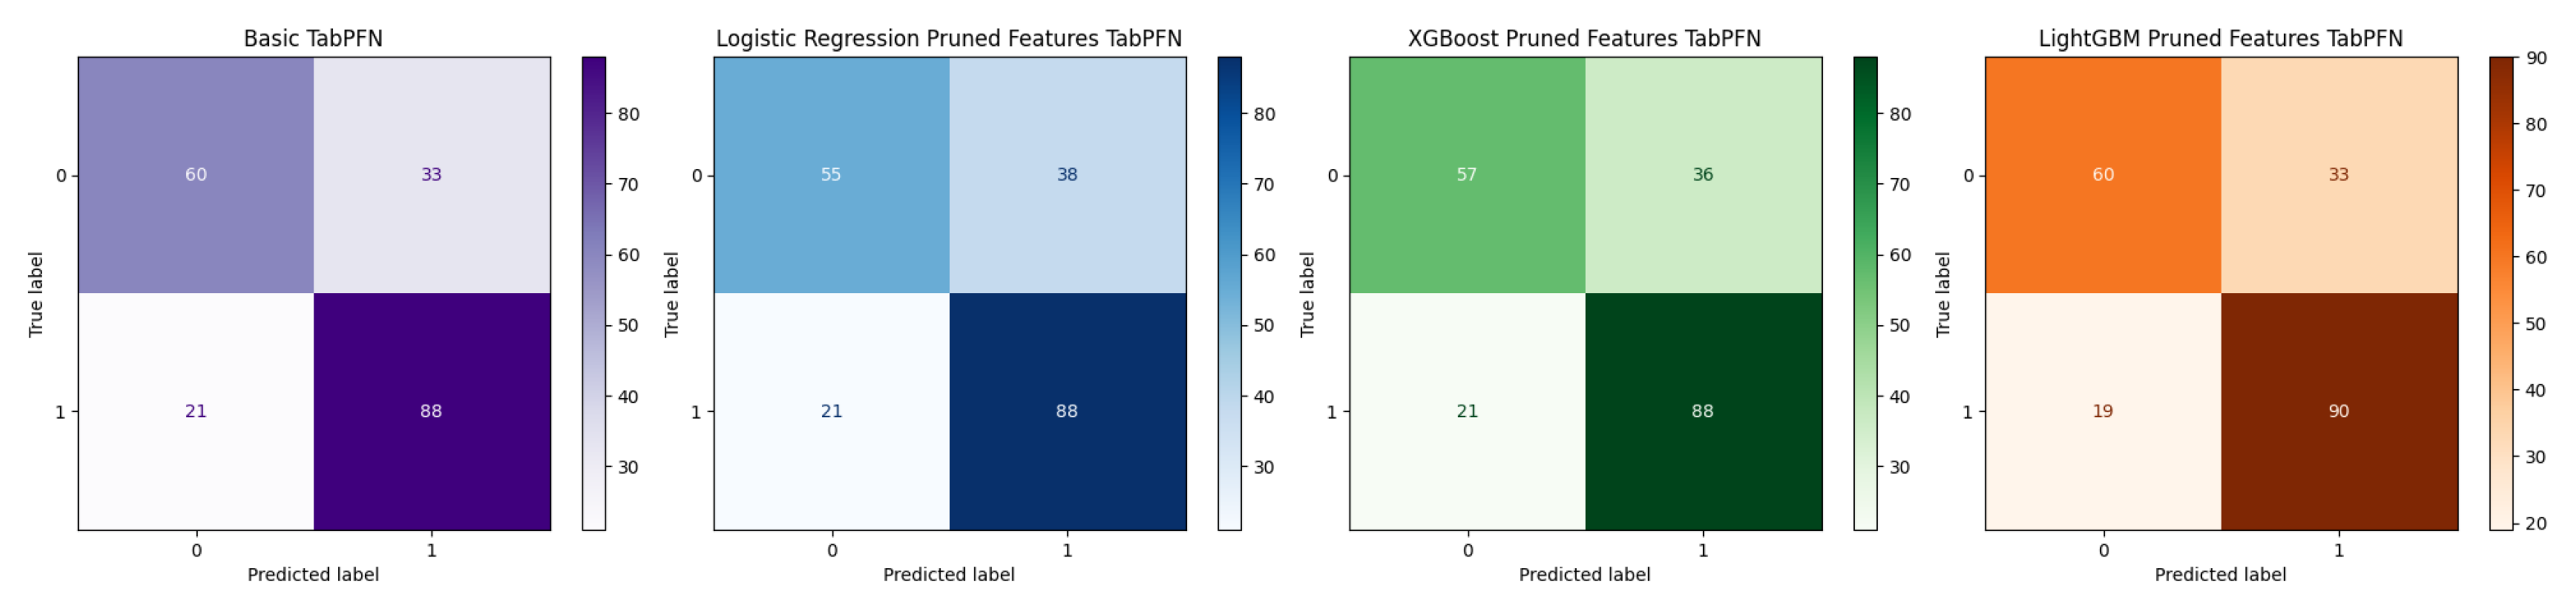
\includegraphics[width=1\linewidth]{TabPFN_confusion_matrices.png}
    \caption{Comparison of confusion matrices on the test set for TabPFN using different feature subsets: (a) Basic TabPFN with all features, (b) TabPFN with Logistic Regression pruned features, (c) TabPFN with XGBoost pruned features, and (d) TabPFN with LightGBM pruned features. Note the slight reduction in false positives (top-right cell) in (d) compared to (a), as mentioned in the text. Values indicate counts for True Negatives, False Positives, False Negatives, and True Positives.}
    \label{fig:TabPFN_confusion_matrices}
\end{figure}

\begin{table}[H]
\centering
\begin{tabular}{lcccc}
\hline
\textbf{Model} & \textbf{Accuracy} & \textbf{AUC} & \textbf{Log-Loss} & \textbf{AP} \\
\hline
Basic TabPFN                                       & 0.733 & 0.835 & 0.487 & 0.875 \\
TabPFN with Logistic Regression pruned features    & 0.708 & 0.826 & 0.505 & 0.860 \\
TabPFN with LightGBM pruned features               & 0.743 & 0.835 & 0.489 & 0.867 \\
TabPFN  with XGBoost pruned features               & 0.718 & 0.824 & 0.500 & 0.862 \\
\hline
\end{tabular}
\caption{Performance comparison of a basic and a feature subset trained models on the test set, evaluated using Accuracy, AUC, Log-Loss, and AP.}
\label{tab:TabPFN_comparison_table}
\end{table}

\section{Robustness Check (added October 2026)}
All results in Section~6 come from a single random 80/20 split. Three questions were left open: how much a single split can vary, whether random splitting flatters the models (maps from the same match can appear in both training and test data, and later matches can be used to predict earlier ones), and how much the 142 engineered features add over a much simpler model. To answer them, the models were re-evaluated with the hyperparameters selected in Section~6 under four schemes: (A) the original split; (B) 30 random 80/20 splits; (C) 30 grouped 80/20 splits in which all maps of a match are kept on the same side; and (D) a forward-in-time split, training on the oldest 80\% of matches and testing on the newest 20\% (HLTV match identifiers increase over time). As a simple baseline, a logistic regression was fitted on only two features: the difference in the teams' mean Rating 2.0 and the difference in their map win rates. TabPFN was not included, since it subsamples features at random on every run.

\begin{table}[H]
\centering
\small
\begin{tabular}{lcccccccc}
\hline
 & \multicolumn{2}{c}{(A) Original} & \multicolumn{2}{c}{(B) 30 random} & \multicolumn{2}{c}{(C) 30 grouped} & \multicolumn{2}{c}{(D) Forward} \\
\textbf{Model} & Acc. & AUC & Acc. & AUC & Acc. & AUC & Acc. & AUC \\
\hline
Two-feature LogReg & 0.693 & 0.787 & 0.707 & 0.791 & 0.715 & 0.797 & 0.694 & 0.801 \\
L1 LogReg          & 0.733 & 0.801 & 0.704 & 0.789 & 0.708 & 0.794 & 0.738 & 0.808 \\
XGBoost            & 0.733 & 0.815 & 0.720 & 0.804 & 0.726 & 0.808 & 0.744 & 0.826 \\
LightGBM           & 0.743 & 0.808 & 0.717 & 0.800 & 0.721 & 0.804 & 0.731 & 0.828 \\
\hline
\end{tabular}
\caption{Accuracy and AUC under four evaluation schemes. (B) and (C) are means over 30 splits; their standard deviations are 0.02-0.03 for both metrics. Majority-class accuracy is 0.54 overall and 0.56 on the forward test set. The tree models were re-run with current library versions, so scheme (A) differs slightly from the tables in Section~6.}
\label{tab:robustness}
\end{table}

Three findings follow from Table~\ref{tab:robustness}. First, the result is robust: accuracy around 72\% and AUC around 0.80 hold across repeated splits, with matches kept intact, and when predicting newer matches from older ones. Second, a single split is noisy: across the 30 random splits, the accuracy of XGBoost ranged from 64.9\% to 77.7\%, so the differences between the tuned models in Section~6 are within sampling noise. Third, the two-feature baseline captures most of the signal. Under repeated splits it is within about one percentage point of accuracy of the 142-feature models, and on the forward split the full feature set adds about four points of accuracy and 0.03 AUC.

Finally, the pruning step was repeated over the 30 grouped splits of scheme (C), choosing features either on the test set, as in Section~6, or on a held-out part of the training data only. With test-set selection, pruned LightGBM reached 74.1\% accuracy and an AUC of 0.828; with training-data selection it reached 71.9\% and 0.807, no better than the unpruned model. The pruning gains reported in Section~6 are therefore an artefact of using the test set for feature selection.

\section{Conclusion}
This project set out to predict Counter-Strike 2 match outcomes from short-term (90-day), map-specific player statistics and to evaluate advanced machine learning models, including the Transformer-based TabPFN. The methodology involved aggregating detailed player performance metrics into team-level summary statistics (mean, standard deviation, sum, minimum, maximum) and comparing the efficacy of tuned Logistic Regression, LightGBM, XGBoost, and TabPFN models.

The models reach about 72\% accuracy and an AUC of 0.80 under repeated held-out evaluation, and this holds when training on older matches and testing on newer ones. Metrics such as kill/death ratio, team map win rates, deaths per round, and HLTV Rating 2.0 were consistently identified as important predictors. However, the robustness check in Section~7 shows that a two-feature model using only rating and map win-rate differences captures most of this performance, so on this dataset the engineered features add little beyond those two signals. The large gains originally attributed to feature pruning (up to 79.7\% accuracy for LightGBM) came from selecting features on the test set and do not hold when the selection uses training data only.

TabPFN delivered competitive performance, with the best log-loss on the original split, without requiring hyperparameter tuning, which supports its use as a strong default for small tabular problems. The overall accuracy is in line with the 71\% reported by the dataset's author and above the 60-65\% reported in the cited CS:GO literature, but those studies used far larger datasets and in some cases out-of-time test sets, so the comparison is indicative rather than direct.

These results must be interpreted with caution due to the small dataset (1010 maps from 577 matches) and restricted time frame (November 2023 - January 2024). The observed accuracy might be specific to the competitive meta and team dynamics of this period and requires validation on larger, more temporally diverse datasets.

Future work should prioritize validating these models and feature engineering strategies on expanded datasets covering longer time periods and potentially different tiers of play, with feature selection carried out inside cross-validation. Investigating additional feature types, such as in-game economic indicators or player role specializations, as well as an Elo-type rating system such as TrueSkill 2, could offer further performance improvements.

In summary, map-specific player statistics support a solid and reproducible predictive model for CS2 match outcomes, and most of its signal can be traced to team rating and map win-rate differences. Careful evaluation - repeated splits, forward-in-time testing, and keeping the test set out of feature selection - proved as important as the choice of model.

% \begin{table}[ht]
% \centering
% \begin{tabular}{lcccc}
% \hline
% \textbf{Model} & \textbf{Accuracy} & \textbf{AUC} & \textbf{Log-Loss} & \textbf{AP Score} \\
% \hline
% Basic Logistic Regressor       & 0.703 & 0.782 & 0.559 & 0.826 \\
% Tuned Logistic Regressor       & 0.733 & 0.801 & 0.548 & 0.847 \\
% Basic LightGBM                 & 0.728 & 0.814 & 0.657 & 0.844 \\
% Tuned LightGBM                 & 0.733 & 0.815 & 0.746 & 0.852 \\
% Pruned LightGBM                & 0.797 & 0.862 & 0.569 & 0.889 \\
% Basic XGBoost                  & 0.733 & 0.799 & 0.558 & 0.830 \\
% Tuned XGBoost                  & 0.719 & 0.815 & 0.536 & 0.850 \\
% Pruned XGBoost                 & 0.777 & 0.834 & 0.513 & 0.871 \\
% TabPFN                         & 0.728 & 0.837 & 0.484 & 0.875 \\
% \hline
% \end{tabular}
% \caption{Performance comparison of different models on evaluation metrics: Accuracy, AUC Score, Log Loss, and Average Precision (AP) Score.}
% \label{tab:model_comparison}
% \end{table}


\bibliographystyle{unsrt}
\bibliography{references}

\end{document}